\newpage
\section{Differential Geometry Primer}
网格参数化
\subsection{Parameterization}
\begin{figure}[!htb]
    \centering
    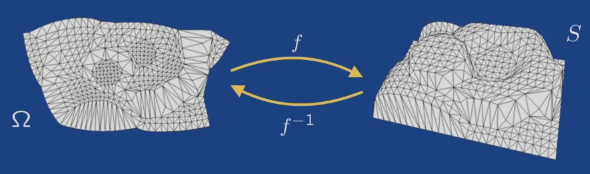
\includegraphics[width=0.42\textwidth]{pic/ACG2/Parameterization}
    \caption{Parameterization}
\end{figure}

\begin{itemize}
    \item Surface $S\subset \R^3$ (开放曲面, 有边界)
    \item Parameter domain $\Omega\subset \R^2$
    \item mapping $f:\Omega\to S$ and $f^{-1}:S\to \Omega$
\end{itemize}

\subsection{Example}
Cylindrical Coordinates:
\begin{itemize}
    \item $S:\{ (x,y,z)\in \R^3: x^2+y^2=1, z\in[0,1] \}$
    \item $\Omega=\{ (\phi, h)\in \R^2:\phi\in[0,2\pi), h\in[0,1] \}$
    \item $f(\phi, h)=(\sin\phi, \cos\phi, h)$
\end{itemize}

Orthographic Projection:
\begin{itemize}
    \item $S:\{ (x,y,z)\in \R^3: x^2+y^2+z^2=1, z\ge 0 \}$
    \item $\Omega=\{ (u, v)\in \R^2:u^2+v^2\le 1 \}$
    \item $f^{-1}(x,y,z)=(x,y)$
    \item $f(u,v)=(u,v,\sqrt{1-u^2-v^2})$
\end{itemize}

\begin{figure}[!htb]
    \centering
    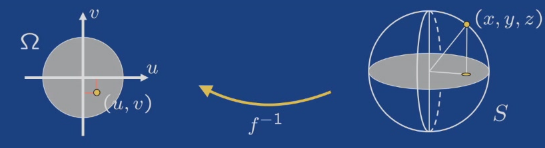
\includegraphics[width=0.42\textwidth]{pic/ACG2/Orthographic Projection}
    \caption{Orthographic Projection}
\end{figure}

Stereographic Projection:
\begin{itemize}
    \item $S:\{ (x,y,z)\in \R^3: x^2+y^2+z^2=1, z\ge 0 \}$
    \item $\Omega=\{ (u, v)\in \R^2:u^2+v^2\le 1 \}$
    \item $f^{-1}(x,y,z)=\left( \frac{x}{1+z}, \frac{y}{1+z} \right)$
    \item $f(u,v)=\left( \frac{2u}{1+u^2+v^2}, \frac{2v}{1+u^2+v^2}, \frac{1-u^2-v^2}{1+u^2+v^2} \right)$
\end{itemize}

\begin{figure}[!htb]
    \centering
    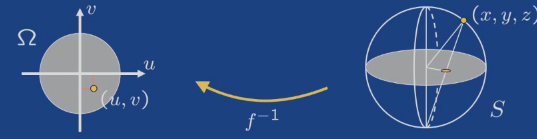
\includegraphics[width=0.42\textwidth]{pic/ACG2/Stereographic Projection}
    \caption{Stereographic Projection}
\end{figure}

Mapping of the Earth

\subsection{Distortion is almost inevitable}
\begin{theorem}[Theorema Egregium]
    A general surface cannot be parameterized without distortion.
\end{theorem}

\begin{itemize}
    \item no distortion = conformal(保角) + equiareal(等面积) = isometric(等测度)
    \item requires surface to be developable(可伸展)
    \subitem planes
    \subitem cones
    \subitem cylindrical
\end{itemize}

\subsection{Distortion}
\begin{itemize}
    \item parameter point $x=(u,v)\in\Omega$
    \item surface point $p=f(x)\in S$
    \item small disk $D(x,r)$ around $x$
    \begin{align*}
        D=D(x,r)=\{ y\in\Omega:\norm{x-y}\le r \}
    \end{align*}
    \item image(像) of $D$ under $f$
    \begin{align*}
        f(D)=\{ f(y):y\in D \}\subset S
    \end{align*}
    \item shape of $f(D)$
\end{itemize}

\begin{figure}[!htb]
    \centering
    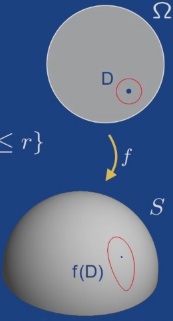
\includegraphics[width=0.22\textwidth]{pic/ACG2/Distortion}
    \caption{Distortion}
\end{figure}

\subsection{Linearization}
\begin{itemize}
    \item $f_u, f_v$ 分别是 $f$ 对 $u,v$ 的偏导
    \item Jacobian of $f$, 这里直接取在 $x$ 的值
    \begin{align*}
        J_f=\left[f_u, f_v\right]\in\R^{3\times 2}
    \end{align*}
    \item tangent plane at $p$
    \begin{align*}
        T_p=\{ p+\alpha f_u+\beta f_v: \alpha,\beta \in \R \}
    \end{align*}
    \item Taylor expansion of $f$
    \begin{align*}
        f(y)=f(x)+J_f(y-x)+\cdots
    \end{align*}
    \item first order approximation of $f$
    \begin{align*}
        g(y)=p+J_f(y-x)\in T_p
    \end{align*}
\end{itemize}

\begin{figure}[!htb]
    \centering
    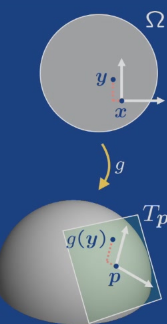
\includegraphics[width=0.22\textwidth]{pic/ACG2/Linearization}
    \caption{Linearization}
\end{figure}

\subsection{Infinitesimal Dis(k)tortion}
\begin{itemize}
    \item small disk $D(x,r)$ around $x$
    \item image of $D$ under $g$
    \begin{align*}
        g(D)=\{ g(y):y\in D \}\subset T_p
    \end{align*}
    \item shape of $g(D)$
    \subitem ellipse
    \subitem semi-axes(半轴) $r\sigma_1$ and $r\sigma_2$
    \item behavior in the limit
    \begin{align*}
        \lim_{r\to 0}g(D)=f(D)
    \end{align*}
\end{itemize}

\begin{figure}[!htb]
    \centering
    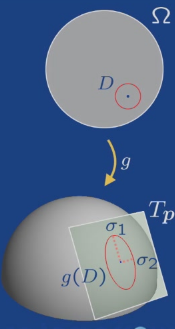
\includegraphics[width=0.22\textwidth]{pic/ACG2/Infinitesimal Dis(k)tortion}
    \caption{Infinitesimal Dis(k)tortion}
\end{figure}

\subsection{Linear Map Surgery}
\begin{itemize}
    \item Singular Value Decomposition (SVD) of $J_f$
    \begin{align*}
        J_f= U\Sigma V^\top =U \begin{pmatrix}
            \sigma_1 & 0 \\ 0 & \sigma_2 \\ 0 & 0
        \end{pmatrix}V^\top
    \end{align*}
    with rotations $U\in \R^{3\times 3}$ and $V\in\R^{2\times 2}$ and scale factors (singular value) $\sigma_1\ge \sigma_2>0$
\end{itemize}

\begin{figure}[!htb]
    \centering
    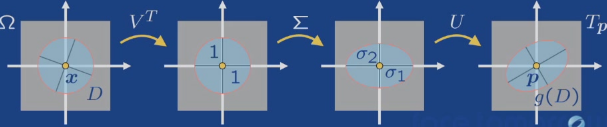
\includegraphics[width=0.42\textwidth]{pic/ACG2/Linear Map Surgery}
    \caption{Linear Map Surgery}
\end{figure}

\subsection{Notion of Distortion}
\begin{itemize}
    \item isometric or length-preserving
    \subitem $\sigma_1=\sigma_2=1$
    \item conformal or angle-preserving
    \subitem $\sigma_1=\sigma_2$
    \item equiareal or area-preserving
    \subitem $\sigma_1\cdot\sigma_2=1$
\end{itemize}
everything defined pointwise on $\Omega$

\subsection{Example}
Cylindrical Coordinates:
\begin{itemize}
    \item $f(\phi, h)=(\sin\phi, \cos\phi, h)$
    \item $J_f=\begin{pmatrix}
        \cos\phi & 0 \\ -\sin\phi & 0 \\ 0 & 1
    \end{pmatrix}, \sigma_1=\sigma_2=1$ (isometric)
\end{itemize}

Orthographic Projection
\begin{itemize}
    \item $f(u,v)=(u,v,\sqrt{1-u^2-v^2})$
    \item $J_f=\begin{pmatrix}
        1 & 0 \\ 0 & 1 \\ -ud & -vd 
    \end{pmatrix}$ with ...
    \item $\sigma_1=1, \sigma_2=d$ neither conformal nor equiareal
\end{itemize}

Stereographic Projection:
\begin{itemize}
    \item $\sigma_1=\sigma_2$ conformal
\end{itemize}

\subsection{Computing the Stretch Factors}
\begin{itemize}%TODO 补充
    \item first fundamental form $I_f$
    \item eigenvalues of $I_f$
    \item singular values of $J_f$
\end{itemize}

\subsection{Measuring Distortion}
\begin{itemize}
    \item loacl distortion measure
    \begin{align*}
        E&:(\R_+\times \R_+)\to \R\\
        (\sigma_1, \sigma_2)&\mapsto E(\sigma_1, \sigma_2)
    \end{align*}
    \item $E$ has minimum at 
    \begin{itemize}
        \item $(\sigma_1, \sigma_2)=(1,1)$ isometric measure
        \item $(\sigma_1, \sigma_2)=(x,x)$ conformal measure
    \end{itemize}
    \item overall distortion
    \begin{align*}
        E(f)=\int_{\Omega}E(\sigma_1(u,v),\sigma_2(u,v))du\ dv\bigg/ Area(\Omega)
    \end{align*}
\end{itemize}

\subsection{Example}%TODO 补充

Conformal Measures
\begin{itemize}
    \item Conformal energy
    \begin{align*}
        E_C=(\sigma_1-\sigma_2)^2/2
    \end{align*}
    \item MIPS energy
    \begin{align*}
        E_M=\kappa_F(J_f)=\norm{J_f}_F\norm{J_f^{-1}}_F=\frac{\sigma_1}{\sigma_2}+\frac{\sigma_2}{\sigma_1}
    \end{align*}
\end{itemize}

isometric Measures
\begin{itemize}
    \item Green-Lagrange deformation tensor
    \item Combined energy
\end{itemize}

Other Measures
\begin{itemize}
    \item Dirichlet energy
    \item Stretch energies
\end{itemize}

\subsection{Piecewise Linear Parameterizations}

\begin{itemize}
    \item piecewise linear atomic maps $f|_t:t\to T$
    \item distortion constant per triangle (因为映射是线性的, 求偏导得 $J_f$ 得 distortion 就是常数)
    \item overall distortion
    \begin{align*}
        E(f)=\sum_{t\in\Omega}E(t)A(t)\bigg/\sum_{t\in\Omega}A(t)
    \end{align*}
\end{itemize}

\begin{figure}[!htb]
    \centering
    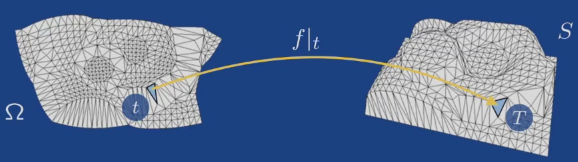
\includegraphics[width=0.42\textwidth]{pic/ACG2/Piecewise Linear Parameterizations}
    \caption{Piecewise Linear Parameterizations}
\end{figure}

\subsection{Beyond Distortion}
\begin{itemize}
    \item surface normal 
    \item surface area
    \item independent of the particular parameterization
    \item intrinsic surface properties
\end{itemize}

\subsection{Curvature}
\begin{itemize}
    \item second fundamental form
    \item Gaussian curvature
    \item mean curvature
\end{itemize}

\subsection{Triangle Mesh Parameterization}
\begin{itemize}
    \item triangle mesh $S\subset \R^3$
    \subitem vertices $p_1,\dots,p_{n+b}$ ($n$个内部点, $b$个边界点)
    \subitem triangles $T_1,\dots,T_m$
    \item parameter mesh $\Omega\subset \R^2$
    \subitem parameter points $u_1,\dots,u_{n+b}$ 
    \subitem parameter triangles $t_1,\dots,t_m$
    \item parameterization $f:\Omega\to S$
    \subitem piecewise linear map $f(t_j)=T_j$
\end{itemize}
\begin{figure}[!htb]
    \centering
    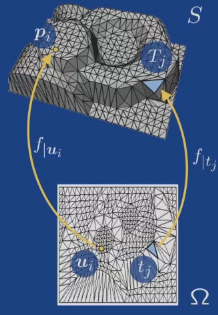
\includegraphics[width=0.22\textwidth]{pic/ACG2/Triangle Mesh Parameterization}
    \caption{Triangle Mesh Parameterization}
\end{figure}

\subsection{The Spring Model}
\begin{itemize}
    \item replace edges by springs
    \item fix boundary vertices
    \item relaxation process
    \item energy of spring between $p_i$ and $p_j$: 
    \begin{align*}
        \frac{1}{2}D_{ij}s_{ij}^2
    \end{align*}
    where spring constant $D_{ij}>0$, spring length $s_{ij}=\norm{u_i-u_j}$
    \item total energy 
    \begin{align*}
        E=\sum_{(i,j)\in\epsilon}\frac{1}{2}D_{ij}\norm{u_i-u_j}^2
    \end{align*}
\end{itemize}

\subsection{Energy Minimization}
\begin{itemize}
    \item interior vertices $p_1,\dots,p_n$
    \item $p_i$'s neighbours $p_j$, $j\in N_i$
    \item overall spring energy
    \begin{align*}
        E=\frac{1}{2}\sum_{i=1}^n\sum_{j\in N_i}\frac{1}{2}D_{ij}\norm{u_i-u_j}^2
    \end{align*}
    \item partial derivative
    \begin{align*}
        \pard{E}{u_i}=\sum_{j\in N_i}D_{ij}(u_i-u_j)
    \end{align*}
    \item minimum of spring energy $E$
    \begin{align*}
        \sum_{j\in N_i}D_{ij}u_i=\sum_{j\in N_i}D_{ij}u_j
    \end{align*}
    for all interior points $u_i, i=1,\dots,n$
    \item $u_i$ is a convex combination of its neighbours $u_j$
    \begin{align*}
        u_i=\sum_{j\in N_i}\lambda_{ij}u_j
    \end{align*}
    with weights $\displaystyle \lambda_{ij}=D_{ij}\bigg/ \sum_{k\in N_i}D_{ik}$
\end{itemize}

\begin{figure}[!htb]
    \centering
    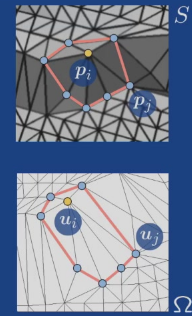
\includegraphics[width=0.22\textwidth]{pic/ACG2/Energy Minimization}
    \caption{Energy Minimization}
\end{figure}


\subsection{The Linear System}
\begin{itemize}
    \item separation of vriables
    \begin{align*}
        u_i-\sum_{j\in N_i, j\le n}\lambda_{ij}u_j=\sum_{j\in N_i, j> n}\lambda_{ij}u_j=\bar{u}_i
    \end{align*}
    \item linear system
    \begin{align*}
        \begin{pmatrix}
            1 & * & \cdots & -\lambda_{ij}\\
            * & 1 & * & \vdots\\
            \vdots & * & \ddots & *\\
            -\lambda_{ji} & \cdots & * & 1
        \end{pmatrix}\begin{pmatrix}
            u_1 \\ u_2 \\ \vdots \\ u_n
        \end{pmatrix}=\begin{pmatrix}
            \bar{u}_1 \\ \bar{u}_2 \\ \vdots \\ \bar{u}_n
        \end{pmatrix}
    \end{align*}
    \item solve system twice
    \begin{align*}
        AU&=\bar{U}\\
        AV&=\bar{V}
    \end{align*}
    for $u$ and $v$ coordinates of interior parameter points
    \item matrix $A$ is 
    \begin{itemize}
        \item sparse
        \item diagonally dominant
        \item nonsingular
    \end{itemize}
\end{itemize}

\subsection{Choice of Weights}
\begin{itemize}
    \item uniform spring constants
    \subitem $D_{ij}=1, \lambda_{ij}=\frac{1}{\# N_i}$
    \item chordal spring constants
    \subitem $D_{ij}=\frac{1}{\norm{p_i-p_j}}, \lambda_{ij}=\frac{D_{ij}}{\sum_{k=N_i}D_{ik}}$
    \item no fold-overs for convex boundary
    \item no linear reproduction
    \subitem planar meshes are distorted
    \item suppose $S$ is a planar mesh
    \item specify weights $\lambda_{ij}$ such taht
    \begin{align*}
        p_i=\sum_{j\in N_i}\lambda_{ij}p_i
    \end{align*}
    \item barycentric coordinates(质心坐标) of $p_i$
    \item then solving
    \begin{align*}
        u_i=\sum_{j\in N_i}\lambda_{ij}u_j
    \end{align*}
    reproduces $S$
\end{itemize}

\subsection{Barycentric Coordinates}

\subsection{Example}
参数化后会折叠, 不好.

\subsection{The Boundary Mapping}

\subsection{Segmentation and Constraints}
\subsubsection{Segmentation}
Necessary for closed and high genus(高规格) meshes. 

分片来做参数化

Goals: Large Charts $\to$ Low Distortion

\begin{itemize}
    \item Single Charts
    \item Multiple Charts
\end{itemize}

e.g. Iso-charts(使用谱分析算法)

\subsubsection{Constraints}
Enforce specific point-to-point correspondences. 

3D mesh and 2D mesh $\to$ constrained texture mapping

e.g. Texture Montage